\chapter{Fusión y ebullición: los cambios de estado}\label{ch:g4:changes-of-state}

Hace años que sabes que el calor derrite el hielo y hace hervir el
agua. Pero ahora tienes un \omterm{def:g3:temperature-thermometers:temperature}{termómetro} --- y el \omterm{def:g3:temperature-thermometers:temperature}{termómetro} trae una
noticia asombrosa desde dentro del cubo de hielo que \omterm{def:g2:ice-water-steam:meltfreeze}{se derrite}:
mientras el hielo \omterm{def:g2:ice-water-steam:meltfreeze}{se derrite}, la \omterm{def:g3:temperature-thermometers:temperature}{temperatura} \emph{se niega a
moverse}. Vamos a mirar los viejos cambios de estado con ojos nuevos.

\section{Los nombres formales}

Los cambios de estado del agua reciben ahora sus nombres de mayores,
que valen para cualquier sustancia y no solo para el agua. De
\omterm{def:g3:solids-liquids-gases:solid}{sólido} a \omterm{def:g3:solids-liquids-gases:liquid}{líquido}: \emph{fusión}\index{fusión}. De \omterm{def:g3:solids-liquids-gases:liquid}{líquido} otra vez
a \omterm{def:g3:solids-liquids-gases:solid}{sólido}: \emph{solidificación}\index{solidificación} (que en el agua
llamamos congelación). De \omterm{def:g3:solids-liquids-gases:liquid}{líquido} a \omterm{def:g3:solids-liquids-gases:gas}{gas}:
\emph{ebullición}\index{ebullición} cuando ocurre deprisa y con
burbujas grandes, y evaporación cuando ocurre en silencio desde la
superficie. De \omterm{def:g3:solids-liquids-gases:gas}{gas} otra vez a \omterm{def:g3:solids-liquids-gases:liquid}{líquido}: condensación. Todas las
sustancias del mundo --- el agua, el chocolate, el hierro, el oro ---
pueden jugar a este juego, cada una a sus propias \omterm{def:g3:temperature-thermometers:temperature}{temperaturas}.

\begin{definition}[Punto de fusión]\label{def:g4:changes-of-state:melting-point}
El \emph{punto de fusión}\index{punto de fusión} de una sustancia es
la \omterm{def:g3:temperature-thermometers:temperature}{temperatura} a la que \omterm{def:g2:ice-water-steam:meltfreeze}{se derrite} --- y también la
\omterm{def:g3:temperature-thermometers:temperature}{temperatura} a la que el \omterm{def:g3:solids-liquids-gases:liquid}{líquido} vuelve a \omterm{def:g2:ice-water-steam:meltfreeze}{congelarse}. Para el agua
es \qty{0}{\celsius}. Cada sustancia tiene el suyo: el chocolate
\omterm{def:g2:ice-water-steam:meltfreeze}{se derrite} cerca de \qty{34}{\celsius} (la \omterm{def:g3:temperature-thermometers:temperature}{temperatura} de la boca
--- eso no es casualidad, pregúntaselo a cualquier chocolatero), la
cera de las velas cerca de \qty{60}{\celsius} y el hierro solo a
\qty{1538}{\celsius}.
\end{definition}

\begin{definition}[Punto de ebullición]\label{def:g4:changes-of-state:boiling-point}
El \emph{punto de ebullición}\index{punto de ebullición} de una
sustancia es la \omterm{def:g3:temperature-thermometers:temperature}{temperatura} a la que hierve. Para el agua es
\qty{100}{\celsius}. Cada sustancia tiene también el suyo --- por eso
una cocinera cuidadosa puede evaporar todo el agua mientras el aceite
de la misma sartén sigue tranquilamente \omterm{def:g3:solids-liquids-gases:liquid}{líquido}.
\end{definition}

\begin{example}[Leer el mundo con dos números]\label{ex:g4:changes-of-state:reading}
¿Por qué está sólida una tableta de chocolate en la estantería
(\qty{20}{\celsius}) y líquida en tu bolsillo durante una excursión de
verano (\qty{35}{\celsius})? Porque su \omterm{def:g4:changes-of-state:melting-point}{punto de fusión}, cerca de
\qty{34}{\celsius}, está \emph{entre} los dos. Una sustancia está
sólida por debajo de su \omterm{def:g4:changes-of-state:melting-point}{punto de fusión} y líquida por encima
--- hasta su \omterm{def:g4:changes-of-state:boiling-point}{punto de ebullición}, donde se marcha hecha \omterm{def:g3:solids-liquids-gases:gas}{gas}. Dos
números cuentan la historia entera de cualquier sustancia a cualquier
\omterm{def:g3:temperature-thermometers:temperature}{temperatura}.
\end{example}

\section{El termómetro cabezota}

\begin{method}[Mirar cómo se derrite el hielo, bien mirado]\label{met:g4:changes-of-state:watch}
\begin{enumerate}
  \item llena un cuenco de hielo picado o de nieve y planta dentro el
        \omterm{def:g3:temperature-thermometers:temperature}{termómetro}; espera y lee: \qty{0}{\celsius};
  \item lleva el cuenco a la cocina templada y lee el \omterm{def:g3:temperature-thermometers:temperature}{termómetro}
        cada pocos minutos mientras el hielo \omterm{def:g2:ice-water-steam:meltfreeze}{se derrite};
  \item sigue leyendo hasta mucho después de que haya desaparecido la
        última esquirla de hielo.
\end{enumerate}
El informe: durante toda la fusión --- con agua y hielo juntos en el
cuenco --- el \omterm{def:g3:temperature-thermometers:temperature}{termómetro} se queda cabezota en \qty{0}{\celsius}. Solo
cuando \emph{el último} trocito de hielo se ha derretido empieza a
subir la \omterm{def:g3:temperature-thermometers:temperature}{temperatura}.
\end{method}

\begin{proposition}[La ley de la meseta]\label{prop:g4:changes-of-state:plateau}
Mientras una sustancia está cambiando de estado --- fundiéndose o
hirviendo ---, su \omterm{def:g3:temperature-thermometers:temperature}{temperatura} se queda quieta en el hito, por mucho
que trabaje el fogón. Todo el calor que llega se gasta en el propio
cambio de estado y nada en subir. El \omterm{def:g3:solids-liquids-gases:solid}{sólido} y el \omterm{def:g3:solids-liquids-gases:liquid}{líquido} conviven
en el \omterm{def:g4:changes-of-state:melting-point}{punto de fusión}; el \omterm{def:g3:solids-liquids-gases:liquid}{líquido} y el \omterm{def:g3:solids-liquids-gases:gas}{gas}, en el
\omterm{def:g4:changes-of-state:boiling-point}{punto de ebullición}.
\end{proposition}

\begin{omfigure}
\begin{tikzpicture}
\begin{axis}[omaxis, width=10.5cm, height=5.6cm,
    xlabel={tiempo sobre el fogón}, ylabel={temperatura (\unit{\celsius})},
    xtick=\empty, ytick={0,100},
    ymin=-40, ymax=140, xmin=0, xmax=10]
  \addplot[very thick, omDef] coordinates
    {(0,-30) (1.5,0) (3.5,0) (5.5,100) (8.5,100)};
  \addplot[very thick, omThm] coordinates {(8.5,100) (9.6,132)};
  \node[below, font=\small] at (axis cs:2.5,-4) {el hielo se funde: meseta};
  \node[above, font=\small] at (axis cs:7.0,103) {el agua hierve: meseta};
\end{axis}
\end{tikzpicture}

{\small Una olla de hielo sobre un fogón constante, contada por el
\omterm{def:g3:temperature-thermometers:temperature}{termómetro}: la \omterm{def:g3:temperature-thermometers:temperature}{temperatura} sube, se detiene en \qty{0}{\celsius}
mientras el hielo \omterm{def:g2:ice-water-steam:meltfreeze}{se derrite}, vuelve a subir y se detiene en
\qty{100}{\celsius} mientras el agua \omterm{def:g2:ice-water-steam:evapcond}{se evapora} hirviendo. (La última
subida roja pertenece al vapor.)}
\end{omfigure}

\begin{omfigure}
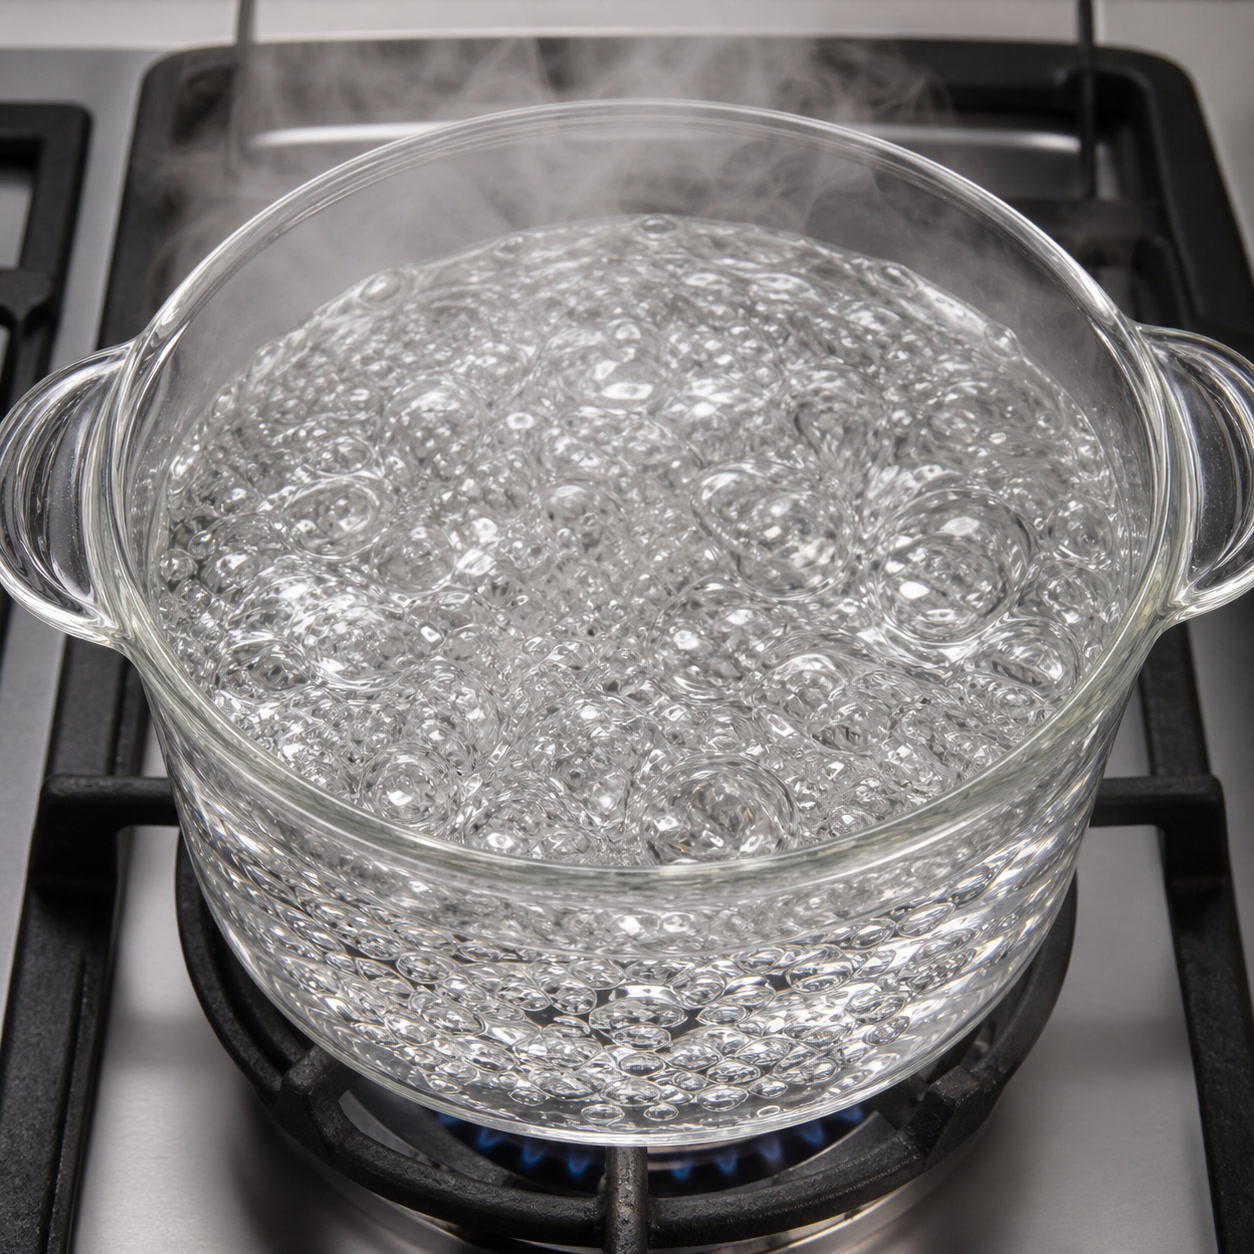
\includegraphics[width=0.45\linewidth]{images/book1/ai/g4-changes-boiling-pot.jpg}

{\small Un hervor a borbotones: dentro del \omterm{def:g3:solids-liquids-gases:liquid}{líquido} se forman burbujas de vapor de agua que revientan en la superficie --- y, mientras tanto, el \omterm{def:g3:temperature-thermometers:temperature}{termómetro} se queda quieto en el \omterm{def:g4:changes-of-state:boiling-point}{punto de ebullición}.}
\end{omfigure}

\begin{example}[La meseta en la cocina]\label{ex:g4:changes-of-state:kitchen}
Por eso el agua que hierve suavemente y la que hierve a borbotones
cuecen la pasta igual de rápido: las dos ollas están exactamente a
\qty{100}{\celsius} --- la furiosa solo malgasta su calor de más
fabricando vapor más deprisa. Y por eso una bebida con cubitos se
queda a \qty{0}{\celsius} hasta la última esquirla: el hielo que se
funde clava la \omterm{def:g3:temperature-thermometers:temperature}{temperatura} en el hito.
\end{example}

\begin{remark}[Un número que el ojo no ve]\label{rem:g4:changes-of-state:invisible}
Sin \omterm{def:g3:temperature-thermometers:temperature}{termómetro}, nadie adivinaría la meseta: la olla parece cada vez
más agitada, el cubo de hielo parece cada vez más tranquilo, y en los
dos la \omterm{def:g3:temperature-thermometers:temperature}{temperatura} está clavada. Es una victoria más de \omterm{def:g2:measuring-length:measure}{medir} sobre
parecer --- y una de las primeras grandes sorpresas que los
instrumentos le regalaron a la ciencia.
\end{remark}

\section{Cada sustancia conserva sus hitos}

\begin{proposition}[Los hitos son marcas de identidad]\label{prop:g4:changes-of-state:identity}
El \omterm{def:g4:changes-of-state:melting-point}{punto de fusión} y el \omterm{def:g4:changes-of-state:boiling-point}{punto de ebullición} de una sustancia
pura no cambian nunca: el agua \omterm{def:g2:ice-water-steam:meltfreeze}{se derrite} a \qty{0}{\celsius} hoy,
mañana, en un palacio o en una tienda de campaña. Los hitos forman
parte de la identidad de la sustancia --- tan bien guardada que un
científico puede reconocer una sustancia desconocida midiendo dónde
\omterm{def:g2:ice-water-steam:meltfreeze}{se derrite} y dónde hierve.
\end{proposition}

\begin{example}[La vela y la fundición]\label{ex:g4:changes-of-state:foundry}
Una vela junto a la chimenea se desploma y gotea: la cera ha pasado su
\omterm{def:g4:changes-of-state:melting-point}{punto de fusión}, cerca de \qty{60}{\celsius}. En una fundición, los
operarios vierten hierro \omterm{def:g3:solids-liquids-gases:liquid}{líquido} de un naranja incandescente como si
fuera sopa --- su horno ha pasado de \qty{1538}{\celsius}. El mismo
juego, con hitos disparatadamente distintos: lo que la chimenea le
hace a la cera, solo un horno se lo puede hacer al hierro. Y el oro
se funde a \qty{1064}{\celsius}: los orfebres conocen ese número, con
las manos si no en grados, desde hace miles de años.
\end{example}

\begin{omfigure}
\begin{tikzpicture}[scale=0.85]
  \draw[-Stealth, very thick] (0.5,0) -- (11.2,0);
  \node[right, font=\small] at (11.15,0.4) {más caliente};
  \foreach \x/\t/\name in {1.3/0/{se funde el hielo}, 3.1/34/{chocolate},
      4.4/60/{cera}, 6.2/100/{hierve el agua}, 8.3/1064/{oro},
      10.1/1538/{hierro}} {
    \draw[thick] (\x,-0.12) -- (\x,0.12);
    \node[above, font=\footnotesize] at (\x,0.2) {$\t$};
    \node[below, font=\footnotesize, align=center] at (\x,-0.2) {\name};
  }
\end{tikzpicture}

{\small Hitos de algunas sustancias cotidianas, en \omterm{def:g3:temperature-thermometers:temperature}{grados Celsius}
(la recta está comprimida --- la marca del hierro está de verdad
quince veces más lejos que la del agua). Cada sustancia lleva siempre
sus propios números.}
\end{omfigure}

\section{Ejercicios}

\begin{exercise}[$\star$]\label{exo:g4:changes-of-state:1}
Di el nombre formal: de \omterm{def:g3:solids-liquids-gases:solid}{sólido} a \omterm{def:g3:solids-liquids-gases:liquid}{líquido}; \ de \omterm{def:g3:solids-liquids-gases:liquid}{líquido} a
\omterm{def:g3:solids-liquids-gases:solid}{sólido}; \ de \omterm{def:g3:solids-liquids-gases:liquid}{líquido} a \omterm{def:g3:solids-liquids-gases:gas}{gas} con burbujas grandes; \ de \omterm{def:g3:solids-liquids-gases:gas}{gas} a
\omterm{def:g3:solids-liquids-gases:liquid}{líquido} en una ventana fría.
\end{exercise}

\begin{exercise}[$\star$]\label{exo:g4:changes-of-state:2}
¿Cuáles son los dos hitos del agua, con sus \omterm{def:g3:temperature-thermometers:temperature}{temperaturas}? ¿Y el
\omterm{def:g4:changes-of-state:melting-point}{punto de fusión} del chocolate, más o menos?
\end{exercise}

\begin{exercise}[$\star$]\label{exo:g4:changes-of-state:3}
Un cuenco contiene hielo y agua juntos, bien removidos. ¿Qué marca el
\omterm{def:g3:temperature-thermometers:temperature}{termómetro}? ¿Qué marcará cinco minutos después, si todavía queda
algo de hielo?
\end{exercise}

\begin{exercise}[$\star$]\label{exo:g4:changes-of-state:4}
Enuncia la ley de la meseta. ¿Adónde va el calor del fogón mientras el
agua hierve, si la \omterm{def:g3:temperature-thermometers:temperature}{temperatura} ya no sube?
\end{exercise}

\begin{exercise}[$\star$]\label{exo:g4:changes-of-state:5}
La cera se funde cerca de \qty{60}{\celsius}. ¿Está una vela
sólida o líquida: en un salón a \qty{20}{\celsius}; \ junto a una
llama que la calienta a \qty{80}{\celsius}; \ en un desván de verano a
\qty{35}{\celsius}?
\end{exercise}

\begin{exercise}[$\star$]\label{exo:g4:changes-of-state:6}
La pasta se cuece en agua que hierve suavemente. Papá pone el fuego al
máximo y la olla hierve a borbotones. ¿Está ahora más caliente el
agua? ¿Qué produce en su lugar el calor de más?
\end{exercise}

\begin{exercise}[$\star$]\label{exo:g4:changes-of-state:7}
En la gráfica de las mesetas del capítulo, ¿cómo puedes localizar los
dos cambios de estado sin leer ni una sola palabra?
\end{exercise}

\begin{exercise}[$\star$]\label{exo:g4:changes-of-state:8}
El hierro se funde a \qty{1538}{\celsius} y el oro a
\qty{1064}{\celsius}. Un horno trabaja a \qty{1200}{\celsius}: ¿cuál
de los dos metales se vierte en él como si fuera sopa y cuál sigue
\omterm{def:g3:solids-liquids-gases:solid}{sólido}? ¿Por cuántos grados se queda corto el horno con el otro?
\end{exercise}

\begin{exercise}[$\star$]\label{exo:g4:changes-of-state:9}
¿Por qué se mantiene igual de fría una bebida con cubitos hasta la
última esquirla de hielo --- y solo entonces empieza a templarse?
\end{exercise}

\begin{exercise}[$\star\star$]\label{exo:g4:changes-of-state:10}
Una científica recibe un \omterm{def:g3:solids-liquids-gases:solid}{sólido} blanco desconocido. Descubre que
se funde exactamente a \qty{0}{\celsius} y que su \omterm{def:g3:solids-liquids-gases:liquid}{líquido} hierve
exactamente a \qty{100}{\celsius}. ¿Cuál es su mejor conjetura sobre
la sustancia --- y qué ley permite que los hitos sirvan de carné de
identidad?
\end{exercise}

\begin{exercise}[$\star\star$]\label{exo:g4:changes-of-state:11}
Los alpinistas cuentan que, allá arriba en las grandes cumbres, el
agua hierve estando \emph{apenas} demasiado caliente para tocarla ---
y que su té nunca sale bien. ¿Qué certeza cotidiana sobre el agua
hirviendo se viene abajo allí arriba? (La razón se esconde en el
propio \omterm{def:g2:air-around-us:air}{aire}, y un capítulo posterior sobre la presión del \omterm{def:g2:air-around-us:air}{aire} la
atrapará.)
\end{exercise}
